\documentclass[a4paper]{article}

\usepackage[a4paper, margin=2.5cm]{geometry}
\usepackage{url}
\usepackage{hyperref}
\usepackage{titlesec}
\usepackage{amsthm}
\usepackage{amssymb}
\usepackage{mathtools}
\usepackage{float}
\usepackage{tikz}
\usetikzlibrary{arrows,automata,positioning}
\usepackage[puttinydots,useemptybox]{braille}

\title{\textbf{Languages, Automata, and Emergent Structure}}
% \date{\today}

\author{
Oliver Turner% - wvdg57 - 001012053
}

\newtheorem{theorem}{Theorem}[section]
\newtheorem{corollary}{Corollary}[section]
\newtheorem{lemma}{Lemma}[section]

\theoremstyle{definition}
\newtheorem{definition}{Definition}[section]
\theoremstyle{definition}
\newtheorem{example}{Example}[section]
\theoremstyle{definition}
\newtheorem{remark}{Remark}[section]


%%%%%%%%%%%%%%%%
\begin{document}
%%%%%%%%%%%%%%%%

\maketitle
\tableofcontents

%%%%%%%%%%%%%%%%%%%%%%%%%%%%%%%%%%%%%%
\section{An Abstraction for Languages}
%%%%%%%%%%%%%%%%%%%%%%%%%%%%%%%%%%%%%%

Mathematics could be described as the study of emergent patterns in abstract structures. As lacking and futile as some might find any attempt at defining something such as Mathematics, this definition does capture some of the activities mathematicians participate in. We often start with a relatively small and simple set of assumptions and then study what they imply and what they allow. We have create sets, vector spaces, categories, groups, and hundreds more abstractions. We have created layers of abstraction by embedding one abstraction into another, what a category theorist might describe as category isomorphisms. Removing unimportant details allows us to generalise, letting us prove facts about \emph{all} functions without having to look at specific ones. Proofs taught in a basic physics course about vectors in space suddenly apply to infinite vector spaces of polynomials. In the following we will look at one such abstraction, \emph{languages}, with particular focus on the class of \emph{automata regular languages}.

\emph{What is a \emph{language}?} The first line from the Wikipedia article describes them as ``a structured system of communication''\footnote{\href{https://en.wikipedia.org/wiki/Language}{Language - Wikipedia - https://en.wikipedia.org/wiki/Language}}. How could we capture this in a mathematical abstraction? It helps to look at some examples of some languages we would like to include in our description:
\begin{itemize}
    \item This is a sentence in English.
    \item \braille{Some English Braille.}
    \item ... --- -- . / -- --- .-. ... .
\end{itemize}

We would also like to include Japanese, Arabic, Nautical flag signaling, programming languages. Even things like postcodes, phone numbers and email addresses are a ``structured system of communication'', albeit they communicate a very specific set of information, so they should be included.

\emph{What do all of these have in common?} They are each a sequence of symbols. These symbols could be visual and colourful like the nautical flags. They could be auditory like Morse code. Yet they are symbols nonetheless. This is the first abstraction we will define, the set of symbols that a languages is defined over and with. It doesn't matter what these symbols are, just that we have a finite set of them to pick from. What is this set of symbols but an alphabet?

\newcommand{\alphabet}{\mathcal{A}}
\begin{definition}
    \label{def:alphabet}
    An \textbf{alphabet} $\alphabet$, is a finite non-empty set containing letters or symbols.
\end{definition}

\begin{remark} Notice that we exclude empty alphabets. What is a language defined with no letters?
\end{remark}

\emph{Concatenating} letters, placing them next to each other in a certain order, gives us words.

\newcommand{\emptyWord}{\varepsilon}
\begin{definition}
    \label{def:word}
    A \textbf{word} $w$, is a concatenations of letters from an alphabet $\alphabet$, representable by a tuple of letters.
    \[
    w := 
    \begin{cases}
        \emptyWord, & \text{if } |w| = 0, \\
        (w_1, w_2, \dots, w_n), w_i \in \alphabet,
        \forall i, & \text{if } |w| > 0,
    \end{cases}
    \]
    Where $|w|$ is the length of the word and $\emptyWord$ is the empty word.
\end{definition}

This already links intuitively with mathematical concepts that we are familiar with such as the Cartesian product: a word $w$ is a tuple of letters from $\alphabet$ of length $n$, so $w \in \alphabet^n$.

A useful concept to define now is the set of all words possible with a certain alphabet. The set containing all words of all lengths possible with the letters from $\alphabet$:

\begin{definition}
    \label{def:aStar}
    The set of all words using an alphabet $\alphabet$ is noted and defined as $\alphabet^* \coloneqq \bigcup\limits_{n \in \mathbb{N}} \alphabet^n$.
\end{definition}

Languages aren't just defined by their alphabet, they have other rules that validate that a word is actually part of that language. For example, although ``pahsdlive'' is a word made with the English alphabet it is not part of the English language. These rules can be as nebulous and flexible as those of English, or as precise as those of a programming language. How do we capture an infinitely flexible set of arbitrarily complex rules? Do we need to? What if we instead focus on what these rules do and what they create. All languages are a new, possibly infinite, set of words made up of this alphabet defined by their rules.

\newcommand{\aLanguage}{\mathcal{L}}
\begin{definition}
    \label{def:language}
    A \textbf{language} on \(\alphabet\) is any subset \(\aLanguage \subseteq \alphabet^*\).
\end{definition}

%%%%%%%%%%%%%%%%%%%%%%%%%
\section{Finite Automata}
%%%%%%%%%%%%%%%%%%%%%%%%%

Languages are complex. It is implausible, and in some senses uninteresting, to analyse all of them at once. The same way we don't analyse all possible functions simultaneously and instead only look at, for example, all continuous functions, we need to impose some restrictions on our languages. Some rules and properties that we can work with to extract patterns. For this purpose let us look at a different concept: \emph{finite automata}.

Our goal is to create a class of languages that can be defined using these finite automata, so what must our automata be capable of? Firstly, they must be able to process our words, they need to accept any character we provide them that is part of our alphabet. Secondly, they must give us a response, some statement of either acceptance into the language or rejection from the language.

Finite automata are also known as finite state machines, this describes slightly more accurately what they consist of: a finite number of internal states, and some way of changing that state through processing an input. We can combine these requirements and properties into the following construct:

\newcommand{\inputAlphabet}{\mathcal{I}}
\newcommand{\automataDef}{(S, S^\prime, \inputAlphabet, T)}
\begin{definition}
    \label{def:fsa}
    A \textbf{finite state automaton} $A := \automataDef$ has four parts:
    \begin{itemize}
        \item A finite non-empty set of internal \textbf{states} $S$;
        \item A subset of states $S^\prime \subseteq S$ designated as \textbf{accepting states};
        \item A finite non-empty set $\inputAlphabet$, called the \textbf{input alphabet}, of input symbols;
        \item A \textbf{transition} or \textbf{next state} function $T : S \times \inputAlphabet \rightarrow S$ that, for each `current state' $s \in S$ and `current input' $i \in \inputAlphabet$ returns a `next state' $T(s,i) \in S$.
    \end{itemize}
\end{definition}

\newcommand{\startStateTable}{\rightarrow}
\newcommand{\acceptStateTable}{\circledcirc}
\begin{example}
    \label{exmp:egAutomata}
    Let us construct a simple automaton \(A = \automataDef\) with:
    \begin{itemize}
        \item Two states, numbered consecutively, \(S = \{1, 2\}\);
        \item One accepting state, \(S^\prime = \{2\}\);
        \item The \emph{binary alphabet} as input alphabet, \(\inputAlphabet = \{0, 1\}\)
        \item A transition function that goes to the state represented by the next input such as the following:
        \begin{align*}
            T : S \times \inputAlphabet &\rightarrow S \\
            (1, 0) &\mapsto 1 \\
            (2, 0) &\mapsto 1 \\
            (1, 1) &\mapsto 2 \\
            (2, 1) &\mapsto 2
        \end{align*}
    \end{itemize}

    We can represent this automata using a \textbf{transition table}. Placing the states along the left and the input alphabet along the top. The values in the table are the state that that row's state transitions to given that column's input. We mark accepting states with a double circle.

    
    \begin{table}[H]
        \centering
        \begin{tabular}{c c | c c} 
          & & 0 & 1 \\
          \hline
           & 1 & 1 & 2 \\ 
          $\acceptStateTable$ & 2 & 1 & 2  \\ 
        \end{tabular}
        \caption{An example transition table.}
        \label{tab:stateTabEx1}
    \end{table}

    This displays the full automata and all of its behaviour, this has similarities to the adjacency matrix for a graph. Like an adjacency matrix we can translate this into a graph to visually represent this table. Figure~\ref{fig:transDiagEx1} is the transition diagram of the automata described in Table~\ref{tab:stateTabEx1}.
    
    %% https://www3.nd.edu/~kogge/courses/cse30151-fa17/Public/other/tikz_tutorial.pdf
    %% https://hayesall.com/blog/latex-automata/
    \begin{figure}[H]
        \centering
        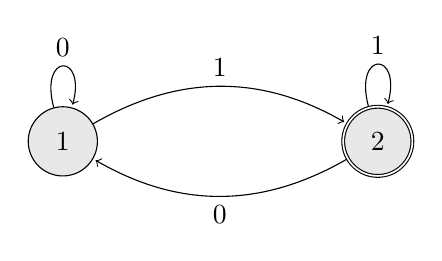
\begin{tikzpicture}[shorten >=1pt,node distance=4cm,auto]
          \tikzstyle{every state}=[fill={rgb:black,1;white,10}]
        
          \node[state]           (a)               {$1$};
          \node[state,accepting] (b) [right of=a]  {$2$};
        
          \path[->]
          (a)   edge [loop above]       node {0} (a)
                edge [bend left, above] node {1} (b)
          (b)   edge [bend left, below] node {0} (a)
                edge [loop above]       node {1} (b);
        \end{tikzpicture}
        \caption{An example transition diagram.}
        \label{fig:transDiagEx1}
    \end{figure}
\end{example}

\emph{How does this process a word?} Given a starting state \(s_0 \in S\) and a word \(w = (w_1, \dots, w_n) \in \inputAlphabet^*\) we can process the word one letter at a time. The state after processing the next letter is always the result of the transition function, given our current state and the next letter. So the state after processing the first letter is \(s_1(w) = T(s_0, w_1)\) and our state after processing all letters up to and including the \(k^\text{th}\) letter is \(s_k(w) = T(s_{k - 1}, w_k)\). This lets us define a function that tells us what state our automaton is after processing a given word.

\begin{definition}
    \label{def:finalStateFn}
    Let $A = \automataDef$ be a finite state automaton and let $w \in \inputAlphabet^*$. For any state $s \in S$, we define the \textbf{final state function}:
    \begin{align*}
        F : S \times \inputAlphabet^* &\rightarrow S \\
        (s, w) &\mapsto s_{\mid w \mid}(w)
    \end{align*}
    
    So $F(s,w)$ is the final state of $A$, started from the initial state $s$, after processing $w$.
\end{definition}

\noindent This now lets us define the language described by our automaton given a specific starting state:

\begin{definition}
    \label{def:langAccepted}
    Let $A = \automataDef$ be a finite state automaton with initial state $s_0$. A word $w \in \inputAlphabet^*$ is \textbf{accepted} by $(A,s_0)$ if $F(s_0,w) \in S^\prime$. The \textbf{language accepted} by $(A, s_0)$, denoted by $\aLanguage(A,s_0)$, is the set of all words that are accepted by $A$ starting from state $s_0$.
\end{definition}

\noindent This lets us, given an automaton, define a language, which in turn lets us describe a class of languages:

\begin{definition}
    \label{def:automatonRegular}
    Given a language $\aLanguage$, on an alphabet $\alphabet$. Then $\aLanguage$ is \textbf{automaton regular} if there exists a finite state automaton, $A$, which has the input alphabet $\alphabet$ and starting state $s_0$ such that $\aLanguage$ is the language accepted by $A$.
\end{definition}

%%%%%%%%%%%%%%%%%%%%%%%%%%%%%%%%%
\section{Operations on Languages}
%%%%%%%%%%%%%%%%%%%%%%%%%%%%%%%%%

Any language $\aLanguage$ on an alphabet $\alphabet$, as defined in Definition~\ref{def:language}, is a set in the universe $\alphabet^*$. This means that standard set operations can be used on languages to define new languages: $\aLanguage_1^\prime$, $\aLanguage_1 \cap \aLanguage_2$, $\aLanguage_1 \cup \aLanguage_2$, $\aLanguage_1 \triangle \aLanguage_2$. \emph{How do these operations affect the \emph{automaton regularity} of languages?}

\begin{lemma}
    \label{lem:compLangReg}
    If the language $\aLanguage$ is \emph{automaton regular} then so is $\aLanguage^\prime$, its \emph{complementary language}.
\end{lemma}
\begin{proof}
    $\aLanguage$ being \emph{automaton regular} means, from Definition~\ref{def:automatonRegular}, that there exists a finite state automaton $A_1 = \automataDef$ and a starting state $s_1$ for which $\aLanguage$ is the \emph{accepted language}. In other words, the final state of the automaton after ``processing'' any word is accepting if and only if that word is in the language $\aLanguage$.
    
    The \emph{complimentary language} of $\aLanguage$, $\aLanguage^\prime$, is made up of every word that is not in $\aLanguage$. To prove \emph{automata regularity} of $\aLanguage^\prime$ we need to construct an automata whose accepting language is $\aLanguage^\prime$.

    Consider the automata $A_2 = (S_1, S_1 \setminus S_1^\prime, \inputAlphabet, T_1)$. As we know, all words in $\aLanguage$ end at a state in $S_1^\prime$ and all words not in $\aLanguage$ end at a state not in $S_1^\prime$. That is, they end at a state in $S_1 \setminus S_1^\prime$, which is the accepting set of $A_2$. This satisfies our condition.

    The result of this process is demonstrated on an example automata in Figure~\ref{fig:automataInvert}.

    \begin{figure}[H]
        \centering
        
        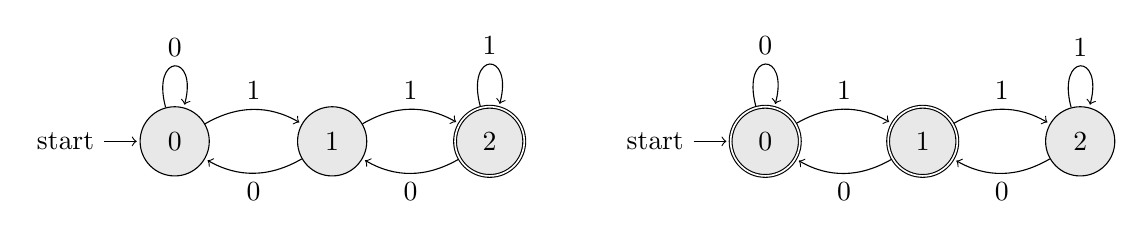
\begin{tikzpicture}[shorten >=1pt,node distance=2cm,auto]
        \begin{scope}
          \tikzstyle{every state}=[fill={rgb:black,1;white,10}]
        
          \node[state,initial]   (a)               {$0$};
          \node[state]           (b) [right of=a]  {$1$};
          \node[state,accepting] (c) [right of=b]  {$2$};
        
          \path[->]
          (a)   edge [loop above]       node {0} (a)
                edge [bend left, above] node {1} (b)
          (b)   edge [bend left, below] node {0} (a)
                edge [bend left, above] node {1} (c)
          (c)   edge [bend left, below] node {0} (b)
                edge [loop above]       node {1} (c);
        \end{scope}
        
        \begin{scope}[xshift=7.5cm]
          \tikzstyle{every state}=[fill={rgb:black,1;white,10}]
        
          \node[state,initial,accepting] (a)               {$0$};
          \node[state,accepting]         (b) [right of=a]  {$1$};
          \node[state]                   (c) [right of=b]  {$2$};
        
          \path[->]
          (a)   edge [loop above]       node {0} (a)
                edge [bend left, above] node {1} (b)
          (b)   edge [bend left, below] node {0} (a)
                edge [bend left, above] node {1} (c)
          (c)   edge [bend left, below] node {0} (b)
                edge [loop above]       node {1} (c);
        \end{scope}
        \end{tikzpicture}
        
        \caption{The right automata is the result of inverting the accepting set of the left automata.}
        \label{fig:automataInvert}
    \end{figure}
    
\end{proof}

\begin{lemma}
    \label{lem:intersectLangsReg}
    If the languages $\aLanguage_1$ and $\aLanguage_2$ are automaton regular over the same alphabet, then the language $\aLanguage_1 \cap \aLanguage_2$, that accepts all of the words accepted by both languages, is also \emph{automaton regular}.
\end{lemma}
\begin{proof}
    The automata constructed for $\aLanguage_1 \cap \aLanguage_2$ is given below:

    \[
    A_3 = (S_1 \times S_2, S_1^\prime \times S_2^\prime, \inputAlphabet, T_3)
    \]
    
    Where $T_3$ is the transition function:
    
    \begin{align*}
        T_3 : (S_1 \times S_2) \times i &\to S_1 \times S_2 \\
            (s_1, s_2, i) &\mapsto (T_1(s_1, i), T_2(s_2, i)) 
    \end{align*}
    
    Verifying that this satisfies Lemma~\ref{lem:intersectLangsReg} is left out for the sake of brevity.
\end{proof}


\begin{theorem}
    \label{thm:setOpsLangReg}
    Using the elementary set operations on automata regular languages $\aLanguage_1$ and $\aLanguage_2$ result in other automata regular languages. 
    
    The elementary set operations are:

    \[
    \aLanguage_1^\prime ,\, \aLanguage_1 \cap \aLanguage_2 ,\, \aLanguage_1 \cup \aLanguage_2 ,\, \aLanguage_1 \triangle \aLanguage_2
    \]
\end{theorem}
\begin{proof}
    The proofs for $\aLanguage_1^\prime$ and $\aLanguage_1 \cap \aLanguage_2$ are Lemma~\ref{lem:compLangReg} and Lemma~\ref{lem:intersectLangsReg} respectively. The other elementary set operations can be constructed using these two\footnote{They form what is known in Boolean logic as a ``universal gate''}.
    
    \begin{align*}
    \aLanguage_1 \cup \aLanguage_2 &\equiv (\aLanguage_1^\prime \cap \aLanguage_2^\prime)^\prime
    \\
    \aLanguage_1 \triangle \aLanguage_2 &\equiv (\aLanguage_1 \cap \aLanguage_2^\prime) \cup (\aLanguage_1^\prime \cap \aLanguage_2)
    \end{align*}

    As all operations used on the right are \emph{automata regularity} preserving, so are the operators on the left.
\end{proof}

%%%%%%%%%%%%%%%%%%%%%%%%%%%%%%%%%%%%%%%%%%%%%%%%%%%%%
\section{The Structure of Languages}
%%%%%%%%%%%%%%%%%%%%%%%%%%%%%%%%%%%%%%%%%%%%%%%%%%%%%

\emph{How does one analyse languages of potentially infinite size?} One step at a time. Instead of looking at all words in a language we look at all words of a certain length. This makes each step a finite analysis as the number of words of length \(n\) is bounded from above by \(|A|^n\) (shown in Lemma~\ref{lem:genFnAStar}). Firstly, let us define a representation for the number of words of a certain length in the language.

\begin{definition}
    The number of words of length \(n\) in the language \(\aLanguage\) is represented by \( c_\aLanguage(n) := |\{ w \in \aLanguage : |w| = n \}| \)
\end{definition}

\begin{definition}
    The \textbf{profile} of a language is the collection of numbers $c_\aLanguage(n)$ for $n = 0,1,2,\dots$.
\end{definition}

\begin{example}
    \label{exmp:langProf}
    Given the language of even base ten numbers. (So using an alphabet of \(\{0, 1, 2, 3, 4, 5, 6, 7, 8, 9\}\)).
    
    \begin{align*}
        c_\aLanguage(0) &= \{ \emptyWord \} &\implies |c_\aLanguage(0)| = 1 \\
        c_\aLanguage(1) &= \{ 0, 2, 4, 6, 8 \} &\implies |c_\aLanguage(1)| = 5 \\
        c_\aLanguage(2) &= \{ 10, 12, 14, \dots, 98 \} &\implies |c_\aLanguage(2)| = 45 \\
        &~\,\vdots
    \end{align*}

    Thus, its profile would be \(1\), \(5\), \(45\), \(450\), \(4500\), \(\dots\).
\end{example}

\begin{definition}
    The \textbf{structure generating function} of a language is the generating function that describes its profile.
    \[
    g_\aLanguage(z) = \sum_{n=0}^\infty z^n c_\aLanguage(n)
    \]
\end{definition}

\begin{example}
    Continuing with the language from Example~\ref{exmp:langProf} its structure generating function would be:
    \[
    g_\aLanguage(z) = 1z^0 + 5z^1 + 45z^2 + 450z^3 + 4500z^4 + \cdots
    \]
\end{example}

\begin{lemma}
    \label{lem:genFnAStar}
    \[
    g_{\alphabet^*}(Z) = \sum_{n=0}^\infty |\alphabet|^n z^n
    \]
\end{lemma}
\begin{proof}
    By definition of the language \(\alphabet^*\) all combinations of letters from \(\alphabet\), no matter the length, is part of the language. So, by induction:

    \noindent Base case: \(n = 0\)

    The only word of length \(0\) in any and all languages is \(\emptyWord\), so \(c_{\alphabet^*}(0) = 1 = |\alphabet|^0\).

    \noindent Inductive step: Assume that \(c_{\alphabet^*}(k) = |\alphabet|^k\), consider the set of words of length \(k + 1\).

    The only way to construct one of these words is to append a letter from \(\alphabet\) to it. For each word of length \(k\) you can choose any letter to append so you have \(|\alphabet|\) choices. So \(c_{\alphabet^*}(k + 1) = |\alphabet| \times |\alphabet|^k = |\alphabet|^{k + 1}\).
    
\end{proof}

Earlier we did set operations on languages and proved what that did to their regularity, but how do they affect the language's structure generating function?

\begin{lemma}
    The sum of the structure generating function of a language and that of its complement is the structure generating function of \(\alphabet^*\).
    \[
    g_\aLanguage(z) + g_{\aLanguage^\prime}(z) = g_{\alphabet^*}(z)
    \]
\end{lemma}
\begin{proof}
    Let us substitute in the definition of \(g\) and the result of Lemma~\ref{lem:genFnAStar}.
    \begin{align*}
        g_\aLanguage(z) + g_{\aLanguage^\prime}(z) &= g_{\alphabet^*}(z) \\
        \sum_{n=0}^\infty z^n c_\aLanguage(n) + \sum_{n=0}^\infty z^n c_{\aLanguage^\prime}(n) &= \sum_{n=0}^\infty |\alphabet|^n z^n \\
        \sum_{n=0}^\infty z^n c_\aLanguage(n) + z^n c_{\aLanguage^\prime}(n) &= \sum_{n=0}^\infty |\alphabet|^n z^n \\
        \sum_{n=0}^\infty z^n (c_\aLanguage(n) + c_{\aLanguage^\prime}(n)) &= \sum_{n=0}^\infty |\alphabet|^n z^n \\
    \end{align*}
    In words, if the number of words of length \(n\) in \(\aLanguage\) plus the number of word of length \(n\) not in \(\aLanguage\) is the total number of words of length \(n\), then we've proven the lemma. This is trivially true.
    
\end{proof}

\begin{lemma}
    \label{lem:genFnOfPrependedLang}
    \[
    \alpha\aLanguage = {\alpha w : w \in \aLanguage}
    \]
    Thus:
    \[
    c_{\alpha\aLanguage}(n) = c_\aLanguage(n-1). % Double check
    \]
    So:
    \[
    g_{\alpha\aLanguage}(z) = z g_\aLanguage(z).
    \]
\end{lemma}

\begin{lemma}
    \label{lem:addOfDisjointGenFn}
    If $\aLanguage_1$ and $\aLanguage_2$ are languages on alphabet $A$ that are disjoint then:
    \[
    g_{\aLanguage_1 \cup \aLanguage_2}(z) = g_{\aLanguage_1}(z) + g_{\aLanguage_2}(z)
    \]
\end{lemma}

%%%%%%%%%%%%%%%%%%%%%%%%%%%%%%%%%%%%%%%%%%%%%%%%%%%%%
\section{The Structure of Automata Regular Languages}
%%%%%%%%%%%%%%%%%%%%%%%%%%%%%%%%%%%%%%%%%%%%%%%%%%%%%

Google became the company that it is today because of their search engine which, originally, functioned on the PageRank algorithm. A simplified version of this algorithm works by creating a matrix, \(M\), that encodes how many times a certain site, \(i\), links to a certain other site, \(j\)\footnote{In reality this is also scaled by a ``trust factor''.} at \(M_{i, j}\). This is seen as the importance of that site. Multiplying \(M\) by itself, repeatedly, propagates the importance of a site to the sites it links to, known as the Eigenvector Centrality of a graph. In other words, if the BBC links to your website, your website becomes more important and trustworthy, this then makes all sites you link to also more trustworthy. Do this for a certain number of iterations and you can sort your search results like Google used to.

Looking at our automata as a graph we could do this to see how many words are in each state after a certain number of iterations using matrix multiplication. Let us define the \textbf{transition matrix} of our automata first:

\begin{definition}
    Given an automata \(A = \automataDef\), let \(M_{i,j}\) be the number of paths (where each input letter is a path) from the state \(i \in S\) to the state \(j \in S\), in other words the number of arrows from \(i\) to \(j\) in the transition diagram. More directly \(M_{i,j} = |\{ \alpha \in \inputAlphabet : T(i, \alpha) = j \}|\).

    So the \textbf{transition matrix} of \(A\) is \(M = (M_{i,j})_{i,j \in S}\)
\end{definition}

\begin{lemma}
    \[ \forall i \in S,\,\sum_{j \in S} M_{i,j} = |\inputAlphabet| \]
\end{lemma}
\begin{proof}
    For any state \(i \in S\), the sum of the row \(i\), \(\sum_{j \in S} M_{i,j}\), is the number of arrows leaving \(i\). Which, as the transition function is complete, is one arrow for each possible input.
\end{proof}

Furthermore, we can show that, given a number of words at a certain state, we can use \(M\) to calculate which state those words go to when processing their next letter.

\begin{lemma} Sure?
    \[
    c_{\aLanguage(A, i)}(n) = \begin{cases}
        0 & \text{if } n = 0 \text{ and } i \notin S^\prime \\
        1 & \text{if } n = 0 \text{ and } i \in S^\prime \\
        \sum_{j \in S} c_{\aLanguage(A, j)}(n - 1) M_{i,j} & \text{if } n > 0.
    \end{cases}
    \]
\end{lemma}
\begin{proof}
    In words, this Lemma is stating that the number of words in the language defined by \(A\), given the starting state \(i\), that are of length \(n\) is the sum of the number of words of length \(n - 1\) for each state that you can get to from \(i\) in one transition.

    Effectively, starting at \(i\), you follow the transition for every possible input letter and ask how many words of length \(n - 1\) start from this state. This is similar to a breadth first search of a graph.

    % TODO

    \noindent \textbf{Base Case}: \(n = 0\) and \(i \notin S^\prime\)

    If \(i\) is not an accepting state there is no word of length \(0\). Hence, \(c_{\aLanguage(A, i)}(0) = 0\).

    \noindent \textbf{Base Case}: \(n = 0\) and \(i \in S^\prime\)

    If \(i\) is an accepting state there is one word of length \(0\), the empty word \(\emptyWord\). Hence, \(c_{\aLanguage(A, i)}(0) = 1\).

    \noindent \textbf{Base Case}: \(n = 1\)

    The words of length one we are considering here have only one symbol, \(w_0\). \(w_0\) is accepting if and only if it transitions into an accepting state, i.e. \(T(i, w_0) \in S^\prime\). The previous base cases mean that the word constructed of this symbol being accepting is equivalent to stating that \(c_{\aLanguage(A, T(i, w_0))}(0) = 1\).
    
    \(\sum_{j \in S} M_{i,j}\) is by definition the number of paths of length \(1\) from state \(i\) to state \(j\). So if the word leading to \(j\) is accepting it is a part of our language and we keep it, i.e. multiply it by \(1 = c_{\aLanguage(A, j)}(0)\). If it is not accepting we ignore it by multiplying by \(0 = c_{\aLanguage(A, j)}(0)\). So \(c_{\aLanguage(A, i)}(1) = \sum_{j \in S} c_{\aLanguage(A, j)}(0) M_{i,j}\).

    \noindent \textbf{Inductive Step}: Assume \( c_{\aLanguage(A, i)}(k) = \sum_{j \in S} c_{\aLanguage(A, j)}(k - 1) M_{i,j} \).

    This can be done using the same logic as the case of \(n = 1\) but instead of relying on the base cases we rely on the inductive step.
    
\end{proof}

We can do this exact same ``vectorisation'' with our structure generating function. We work upwards instead this time which means we don't need to subtract one for each recursion, we simply multiply by \(z\) and keep going until infinity.

\begin{lemma}
    \[
    g_{\aLanguage(A, i)}(z) = c_{\aLanguage(A, i)}(0) + z \sum_{j \in S} g_{\aLanguage(A, i)}(z) M_{i,j}
    \]
\end{lemma}

We can make this more general by considering all states simultaneously.

\begin{definition} Given:
    \[
    v = c_{\aLanguage(A, i)}(0) = 
    \begin{cases}
        1, & \text{if } i \in S^\prime, \\
        0, & \text{if } i \notin S^\prime,
    \end{cases}
    \]
    We call $(v_i)_{i \in S}$ (a column vector) the \textbf{acceptance vector}.
\end{definition}

\begin{theorem}
    \label{thm:vectorized}
    \[
    g(z) = v + z M g(z)
    \]
\end{theorem}

%%%%%%%%%%%%%%%%%%%%%%%%%%%%%%%%%
\section{Structure From Automata}
%%%%%%%%%%%%%%%%%%%%%%%%%%%%%%%%%

Our abstraction of language and our condition of automata regularity have come together rather beautifully to connect with graph theory and linear algebra. Let us explore what Theorem~\ref{thm:vectorized} allows us to do with an example.

\begin{example}
    Consider the automata in Figure~\ref{fig:nonTrivAuto}, a slightly more complex automata than we have looked at previously.

    \begin{figure}[H]
        \centering
        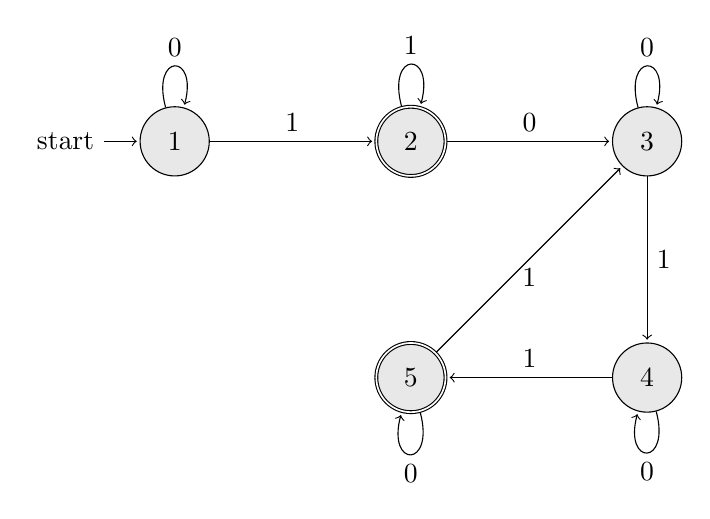
\begin{tikzpicture}[shorten >=1pt,node distance=3cm,auto]
          \tikzstyle{every state}=[fill={rgb:black,1;white,10}]
        
          \node[state,initial]   (a)               {$1$};
          \node[state,accepting] (b) [right of=a]  {$2$};
          \node[state]           (c) [right of=b]  {$3$};
          \node[state]           (d) [below of=c]  {$4$};
          \node[state,accepting] (e) [below of=b]  {$5$};
        
          \path[->]
          (a)   edge [loop above]       node {0} (a)
                edge [above]            node {1} (b)
          (b)   edge [above]            node {0} (c)
                edge [loop above]       node {1} (b)
          (c)   edge [loop above]       node {0} (c)
                edge [right]            node {1} (d)
          (d)   edge [loop below]       node {0} (d)
                edge [above]            node {1} (e)
          (e)   edge [loop below]       node {0} (e)
                edge [below]            node {1} (c);
        \end{tikzpicture}
        \label{fig:nonTrivAuto}
    \end{figure}

    As the accepting states are \(2\) and \(5\) we can easily construct the \emph{acceptance vector}.
    \[
    v = \begin{bmatrix}
           0 \\
           1 \\
           0 \\
           0 \\
           1
         \end{bmatrix}
    \]

    We can also construct our \emph{transition matrix} by observation. Where each state goes to itself once and the next one once, except the last state which goes to \(3\) instead.
    \[
    M = \begin{bmatrix}
           1 & 1 & 0 & 0 & 0 \\
           0 & 1 & 1 & 0 & 0 \\
           0 & 0 & 1 & 1 & 0 \\
           0 & 0 & 0 & 1 & 1 \\
           0 & 0 & 1 & 0 & 1
         \end{bmatrix}
    \]

    These can be simply placed into Theorem~\ref{thm:vectorized} to give us the following equation.
    \begin{align*}
        g(z) &= v + z M g(z) \\[1em]
        \begin{bmatrix}
           g_1(z) \\
           g_2(z) \\
           g_3(z) \\
           g_4(z) \\
           g_5(z)
         \end{bmatrix} &= \begin{bmatrix}
           0 \\
           1 \\
           0 \\
           0 \\
           1
         \end{bmatrix} + z \begin{bmatrix}
           1 & 1 & 0 & 0 & 0 \\
           0 & 1 & 1 & 0 & 0 \\
           0 & 0 & 1 & 1 & 0 \\
           0 & 0 & 0 & 1 & 1 \\
           0 & 0 & 1 & 0 & 1
         \end{bmatrix} \begin{bmatrix}
           g_1(z) \\
           g_2(z) \\
           g_3(z) \\
           g_4(z) \\
           g_5(z)
         \end{bmatrix} \\[1em]
         &= \begin{bmatrix}
           0 \\
           1 \\
           0 \\
           0 \\
           1
         \end{bmatrix} + z \begin{bmatrix}
           g_1(z) + g_2(z) \\
           g_2(z) + g_3(z) \\
           g_3(z) + g_4(z) \\
           g_4(z) + g_5(z) \\
           g_3(z) + g_5(z)
         \end{bmatrix} \\[1em]
        \begin{bmatrix}
           g_1(z) \\
           g_2(z) \\
           g_3(z) \\
           g_4(z) \\
           g_5(z)
         \end{bmatrix} &= \begin{bmatrix}
           z(g_1(z) + g_2(z)) \\
           1 + z(g_2(z) + g_3(z)) \\
           z(g_3(z) + g_4(z)) \\
           z(g_4(z) + g_5(z)) \\
           1 + z(g_3(z) + g_5(z))
         \end{bmatrix}
    \end{align*}

    As our starting states is \(1\) we will use this to find \(g_1\), however, this works for any starting state. By going row by row we get:
    \begin{align*}
        g_1(z) &= zg_1(z) + zg_2(z) \implies \frac{1 - z}{z}g_1(z) = g_2(z) \\
        g_2(z) &= 1 + zg_2(z) + zg_3(z) \implies \frac{1 - z}{z}g_2(z) - 1 = g_3(z) \\
        g_3(z) &= zg_3(z) + zg_4(z) \implies \frac{1 - z}{z}g_3(z) = g_4(z) \\
        g_4(z) &= zg_4(z) + zg_5(z) \implies \frac{1 - z}{z}g_4(z) = g_5(z) \\
        g_5(z) &= 1 + zg_3(z) + zg_5(z) \implies \frac{1 - z}{z}g_5(z) - 1 = g_3(z)
    \end{align*}

    \noindent We can keep substituting these into the last equation to put it in terms of \(g_1(z)\):
    \begin{align*}
        (1 - z)g_5(z) - 1 &= zg_3(z) \\
        (1 - z)\left(\frac{1 - z}{z}g_4(z) - 1\right)
            &= z\left(\frac{1 - z}{z}g_2(z) - 1\right) \\
        \frac{(1 - z)^2}{z}g_4(z) - (1 - z) &= (1 - z)g_2(z) - z \\
        &~\,\vdots ~\longrightarrow~ \text{Full working available in the Appendix}\\
        g_1(z)
            &= \frac{1 - 3z + 3z^2 - 2z^3 + z^6 - z^7}
            {z^2 - 5z^3 + 10z^4 - 11z^5 + 7z^6 - 2z^7} \\
    \end{align*}

    This is an example of a Theorem we won't cover here, which is that: for any automata and starting state, the structure generating function will always be a ratio of polynomials.
\end{example}

\appendix
\section{Extended Working}

\begin{align*}
    (1 - z)g_5(z) - 1 &= zg_3(z) \\
    (1 - z)\left(\frac{1 - z}{z}g_4(z) - 1\right)
        &= z\left(\frac{1 - z}{z}g_2(z) - 1\right) \\
    \frac{(1 - z)^2}{z}g_4(z) - (1 - z) &= (1 - z)g_2(z) - z \\
    \frac{1 - z}{z}g_4(z) - 1 &= g_2(z) - \frac{z}{1 - z} \\
    \frac{1 - z}{z}\frac{1 - z}{z}g_3(z) - 1 &= \frac{1 - z}{z}g_1(z) - \frac{z}{1 - z} \\
    \frac{(1 - z)^2}{z^2}g_3(z) - 1 &= \frac{1 - z}{z}g_1(z) - \frac{z}{1 - z} \\
    \frac{(1 - z)^2}{z^2}\left(\frac{1 - z}{z}g_2(z) - 1\right) - 1
        &= \frac{1 - z}{z}g_1(z) - \frac{z}{1 - z} \\
    \frac{(1 - z)^3}{z^3}g_2(z) - \frac{(1 - z)^2}{z^2} - 1
        &= \frac{1 - z}{z}g_1(z) - \frac{z}{1 - z} \\
    \frac{(1 - z)^3}{z^3}\frac{1 - z}{z}g_1(z) - \frac{(1 - z)^2}{z^2} - 1
        &= \frac{1 - z}{z}g_1(z) - \frac{z}{1 - z} \\
    \frac{(1 - z)^4}{z^4}g_1(z) - \frac{(1 - z)^2}{z^2} - 1
        &= \frac{1 - z}{z}g_1(z) - \frac{z}{1 - z} \\
    g_1(z)\left(\frac{(1 - z)^4}{z^4} - \frac{1 - z}{z}\right)
        &= \frac{(1 - z)^2}{z^2} - \frac{z}{1 - z} + 1 \\
    g_1(z)\frac{(1 - z)^4 - z^3(1 - z)}{z^4}
        &= \frac{(1 - z)^3 - z^3}{z^2(1 - z)} + 1 \\
    g_1(z)
        &= \frac{\frac{z^4((1 - z)^3 - z^3)}{z^6(1 - z)} + z^4}
        {(1 - z)^4 - z^3(1 - z)} \\
    g_1(z)
        &= \frac{z^4((1 - z)^3 - z^3) + z^{10}(1 - z)}
        {z^6(1 - z)^5 - z^9(1 - z)^2} \\
    g_1(z)
        &= \frac{z^4 - 3z^5 + 3z^6 - 2z^7 + z^{10} - z^{11}}
        {z^6 - 5z^7 + 10z^8 - 11z^9 + 7z^{10} - 2z^{11}} \\
    g_1(z)
        &= \frac{1 - 3z + 3z^2 - 2z^3 + z^6 - z^7}
        {z^2 - 5z^3 + 10z^4 - 11z^5 + 7z^6 - 2z^7} \\
\end{align*}

%%%%%%%%%%%%%%
\end{document}
%%%%%%%%%%%%%%


